\beginsong{Nordwärts}[
    wuw={Silke Neumann}, 
    jahr={1982},
    bo={248}, 
    pfii={60}, 
    pfiii={46}, 
    gruen={77}, 
    kssiv={30}, 
    siru={173}, 
    tonspur={422}, 
]

\beginverse
\endverse
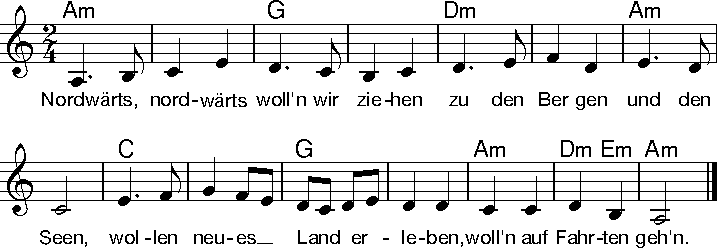
\includegraphics[draft=false, width=1\textwidth]{Noten/Lied072.pdf}	

\beginverse
\[Am]Wollen frei so \[G]wie ein Vogel \[Dm]wiegen uns im \[Am]kalten Wind,
\[C]woll'n den Ruf der \[G]Wildnis hören, \[Am]wenn wir \[Dm]glück\[Em]lich \[Am]sind.
\endverse

\beginverse
^Woll'n durch Moor und ^Sümpfe waten, ^abends legen ^uns zur Ruh'.
^Klampfen sollen ^leis' erklingen, ^singen ^im^mer^zu.
\endverse

\beginverse
^In der Kohte ^brennt ein Feuer, ^füllt uns alle ^mit Bedacht.
^Schlaf senkt sich auf ^uns hernieder, ^doch die ^Wild^nis ^wacht.
\endverse

\beginverse
^Käuzchenschreie, ^Bäume rauschen ^bis zum frühen ^Morgengrau.
^Über ausge^qualmtem Feuer ^strahlt der ^Him^mel ^blau.
\endverse

\beginverse
^Wenn wir wieder ^heimwärts ziehen, ^sehnet jeder ^sich zurück,
^denkt an die ver^gang'nen Fahrten, ^an ver^gang'^nes ^Glück.
\endverse

\beginverse
^Nordwärts, nordwärts ^woll'n wir wieder ^zu den Bergen ^und den Seen,
^dieses Land noch^mal erleben ^und auf ^Fahr^ten ^geh'n.
\endverse


\endsong
